\section{Physarum Polycephalum}
\label{section:background_physarum}

The organism being a subject for this work is \textit{Physarum Polycephalum} also called the many-headed slime mould. It is a member of the \textit{Physaridae} family of slime moulds, in order of \textit{Physarales}, class \textit{Myxogastria}, phylum \textit{Myxomycete}, supergroup \textit{Amoebozoa} in \textit{Protista} kingdom. While current position in taxology is well defined, presented characteristics will justify why scientists used to have problems with classification of the Physarum \cite{stephenson1994myxomycetes}.

In order to make the thesis readable, terms \textit{Physarum Polycephalum}, \textit{Physarum} or \textit{the slime mould} will be used interchangeably as the subject is unambiguously defined. As none of the authors have a background in biology, concepts are presented from a computer scientist's perspective in minimal, yet exhaustive, form.


\subsection{Biological characteristics}

\textit{Physarum Polycephalum} is a very peculiar organism. Even being a \textit{Protista} it can be observed with a naked eye --- it is a one amongst biggest living unicellular ogranisms \cite{TODO}. 

In its natural habitat, under cool, dark and humid conditions the slime mould exists in form of a yellow semistructurized blob (as seen in figure \ref{figure:bp_habitat}). Its occurrence is fairly common around the globe, however species \textit{Physarum Polycephalum} does not occur naturally in Poland \cite{narkiewicz2013grzyby}. It feeds on bacteria, fungi and other sources of basic nutrients.

In labaratory conditions, \textit{Physarum} is stored on Petri dishes filled with non-nutritious agar (figure \ref{figure:bp_petri}). The agar base provides humid environment required for supporting plasmodial stage of the slime mould. A sterille oats or even soft porridge is used as controlled source of nutrients. Complete description of storage and observation protocol, among other informations, is provided in Appendix \ref{chapter:protocol}.

\begin{figure}
  \centering
  % TODO find another image
  \begin{subfigure}{0.45\textwidth}
    \centering
    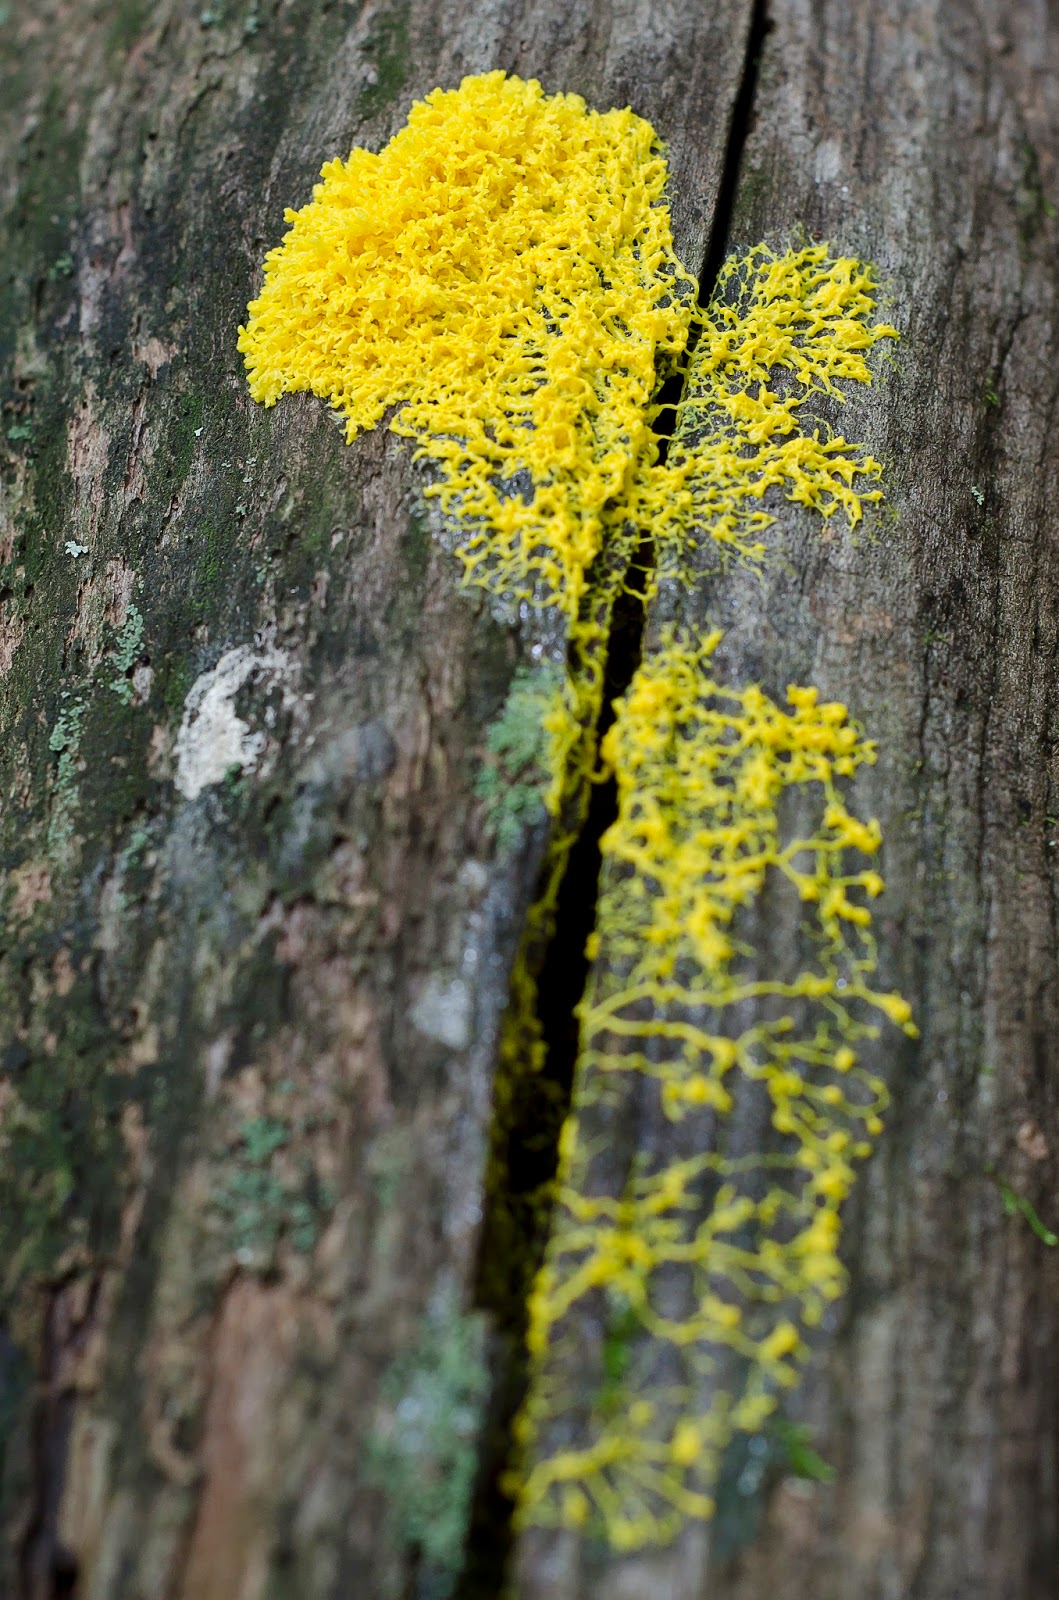
\includegraphics[width=0.44\textwidth]{background/physarum/habitat.jpg}
    \caption{Natural habitat \cite{TODO}}
    \label{figure:bp_habitat}
  \end{subfigure}
  \begin{subfigure}{0.45\textwidth}
    \centering
    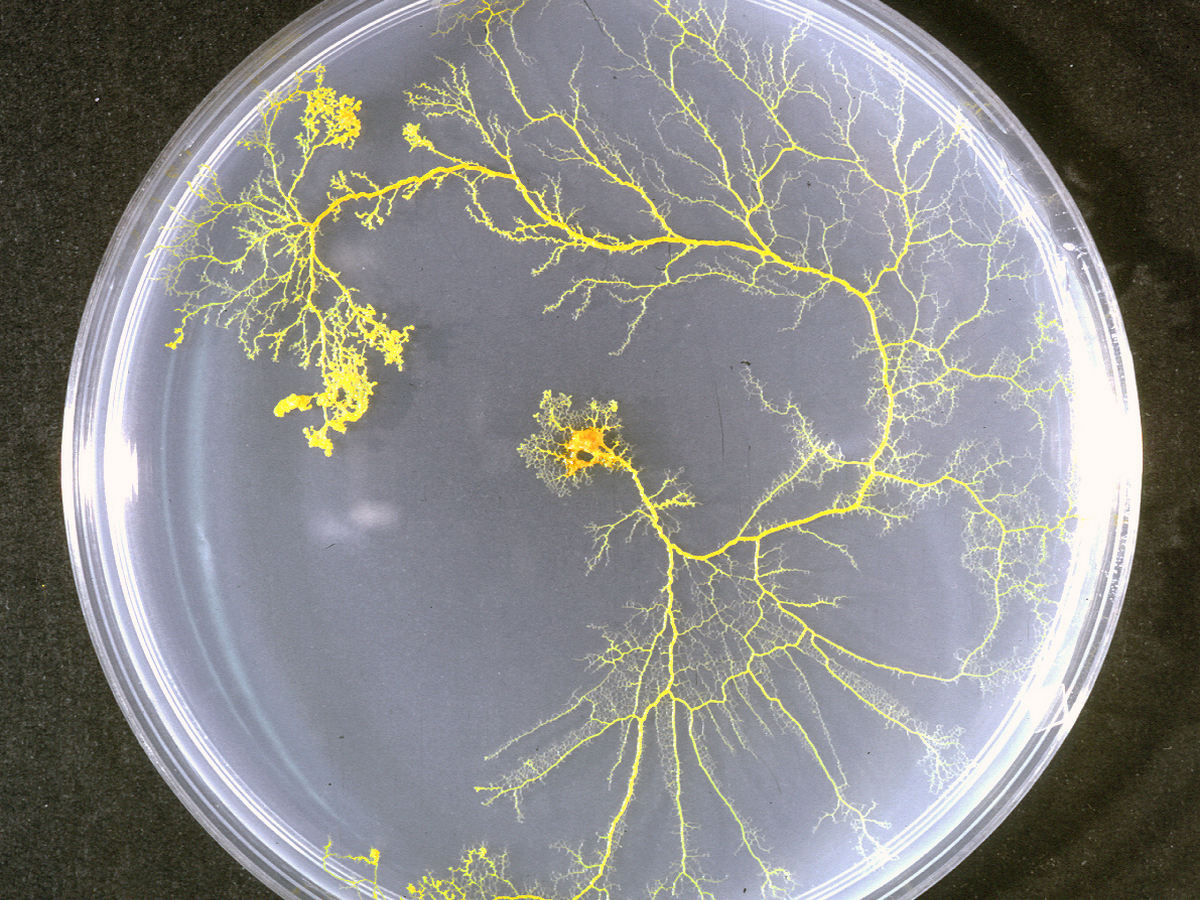
\includegraphics[width=0.9\textwidth]{background/physarum/petri.jpg}
    \caption{Petri dish}
    \label{figure:bp_petri}
  \end{subfigure}
  \caption{\textit{Physarum Polycephalum} in plasodial stage}
\end{figure}

% TODO preferred image from carolina
\begin{figure}
  \centering
  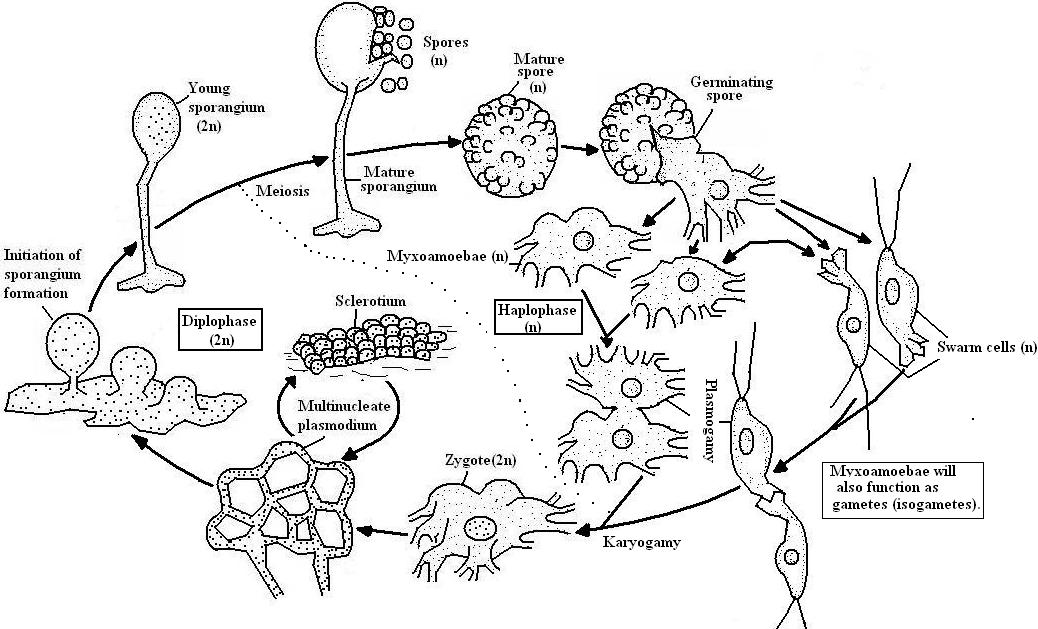
\includegraphics[width=0.94\textwidth]{background/physarum/lifecycle.png}
  \caption{Lifecycle of \textit{Physarum Polycephalum} \cite{TODO}}
  \label{figure:bp_lifecycle}
\end{figure}

As representant of \textit{Myxomycete}, a life cycle of the slime mould is very complex including haploid and diploid phases (as seen in figure \ref{figure:bp_lifecycle}). Such cycle is result of evolutionary adaptation. Formation of sporangium occurs in result of worsening conditions (such as inadequate temperature, humidity or acidity). Sporangium releases spores, which can germinate into ameboid swarm cell. Such cell can enclose itself into a cyst to protect the cells until environmental conditions improve. When conditions are favourable amoeboid cell turns into flagellated swarm cell. Swarm cells can merge, fuse their nuclei and start mitotic process resulting in forming a plasmodium \cite{jones2015pattern}.

% TODO ref
For purposes of unconventional computing applications, \textit{Physarum} is preferred in its such plasmodial stage. However, during research transformations into other states are inevitable and must be dealt with. In case of drying and enforced starvation sclerotium is formed --- in this dormant phase \textit{Physarum Polycephalum} can survive for many years until dampness and nutrients are provided again.

Plasmodium forms protoplasmic tubes accordingly to food availability. Such tubes are used for discovery and transportation of nutrients. The tubes are built in similar way to animal muscles. The ectoplasm contains actin and myosin complexes, which are organised into regular structures forming tubes. Such actomyosin complexes generate contractile motion resulting in streaming of protoplasm. Furthermore, synchronized oscillations of protoplasm stream direction can observed. Nutrients are transported in one direction, after 1-2~minutes the direction is reversed. Period of this oscillation depends on environment quality and accesibility to food \cite{wohlfarth1979oscillatory}. 

The plasmodium can grow around 10~mm per hour when actively exploring environment \cite{coggin1996dynamic}. While moving, plasmodium leaves polysaccharide traces (informally called slime, hence the name slime mould). Network of the protoplasmic tubes adapts to forming efficient ways of transporting nutrients, depending on their amount and quality \cite{nakagaki2004obtaining}. 


\subsection{Observations}

lorem


\subsection{Emerging computational possibilities}

lorem


\subsection{Interaction}

lorem

